% !TeX spellcheck = en_GB
% !TeX spellcheck = en_US 
\chapter{ Data Acquisition and Calibration Methods.}

Taking advantage of the possibility to record individual signal in the TOF and the VMI spectrometer, we develop a method in which the data of both detectors is correlated to describe a single coulomb explosion. The large exposure time of the camera and the software limitations required the use of a trigger protocol in order to collect and sort the signal coming from a single laser shot. The next section present the triggering protocol developed for the ELI-Alps beam time, together to the calibration methods used for the VMI. In addition, in our experiment, in contrast to other spectroscopic techniques, the Photoelectric Spectra (PES) of the $e-$ VMI looks different for each signal because of the size distribution of the clusters production and the different focus intensities each cluster is exposed to. Nevertheless, the images and therefore the PES look rather similar in shape, small circular bloops in the middle of the detector with a clear edges and a brightness higher than the background. The larger clusters ($\langle N \rangle = 10^{6}$) present small deformation in the circles as show in chapter 4. For example, some images show small-medium  uniformly bright circles  while others signal, shows high intensities in the edges and lower in the center, like a "donut", as we will refer from now. In section 3.3 we present the Data  protocol and the algorithms used to detect, sort and analyse the acquired signal.


\begin{figure}[h!]
\centering
\begin{subfigure}[]{0.7\textwidth}
\caption{selected VMI signals for helium in MIR lasers}
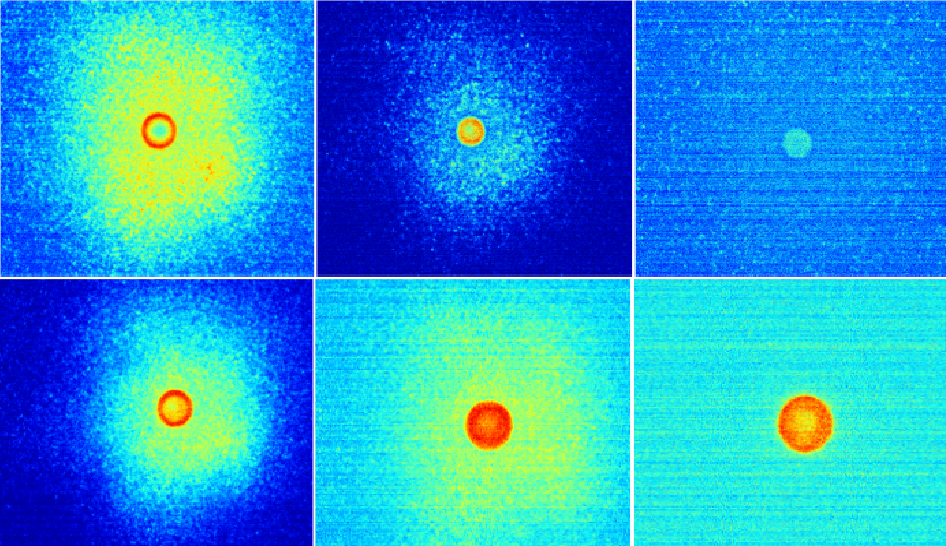
\includegraphics[width=1\textwidth]{../Images/Raw_He_ramdom.png} \end{subfigure} 
\begin{subfigure}[]{0.7\textwidth}
\caption{selected VMI signals for neon in MIR lasers}
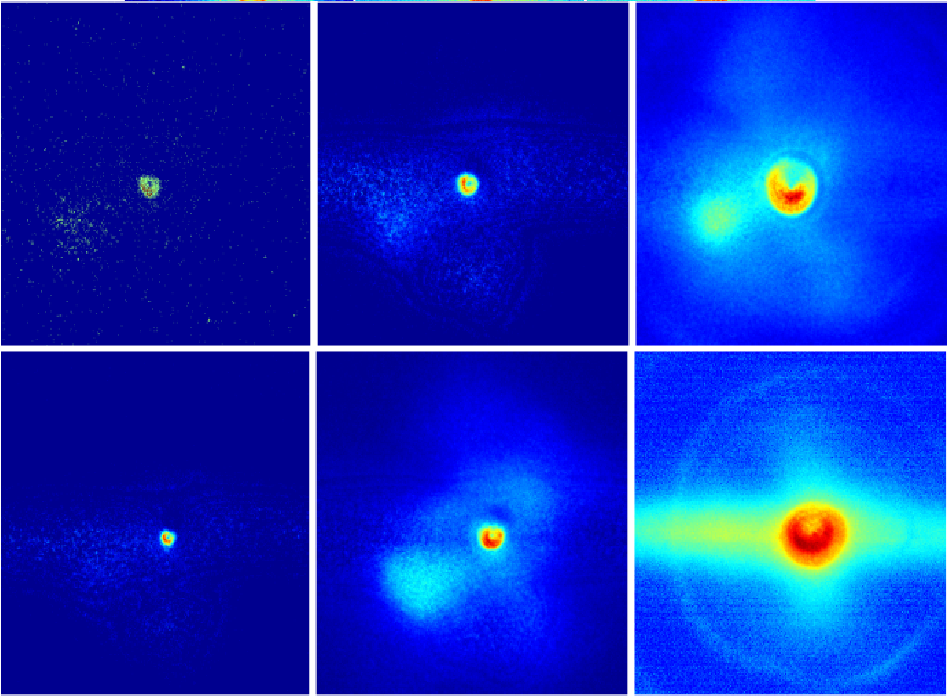
\includegraphics[width=1\textwidth]{../Images/Raw_Ne_ramdom.png} \end{subfigure} 
\caption[VMI raw images example]{Example images of MIR VMI signal in He and Ne with different parameters. On the top, several example plasma signal including, low intensity and the donut shape. On the bottom, random example for Ne signals, including low signal and non-uniform bloops.}
\label{fig:vmiexample}
\end{figure}



\section{Camera and Trigger Protocol}

One of the main objectives of this project, is to record individual data for single shots nanoplasma explosion in the VMI and TOF. The advantage is the ability of the threat the data in a separate way to reduce the background and know the energy distribution information that is lost when data is averaged.

Two methods were developed. A first approach was done using a software triggering for the CCD camera and the oscilloscope, an Acqiris Card CC103, for the TOF. Using Lab View, an external clock (a RasberryPi 3) was triggered by the laser, the beginning of the explosion, at the same time, it software-trigger the camera and oscilloscope programs to start the acquisition. Having all the data acquired in the same software would allow to sort the data online and reduce the storage needed for the experiment. The Lab view program was tested unsuccessfully for the data acquisition rate needed in ELI $100$ KHz, the main problem was that when a software-triggering scheme is used, extra delays are applied due to the operating system and the communication protocols, so even the data were acquired at the same time the delays at saving the information it in the hard drive made impossible to correlate the signals.

Based on that same idea, a second approach was used. As alternative of the software triggering, a hardware triggering was used. The laser triggers a delay generator that at the same time triggers the oscilloscope, a $R.S$ RTO2000 with bandwidth of 600MHZ to 6GHz, and the camera. Two facts need to be taken into account, first, the minimal exposure time of the camera is 34 $\mu$s. Second, the timing between the camera receiving the trigger signal and the real start of the acquisition is not negligible as it is for the oscilloscope. The camera took 5-6 $\mu$s to start after the trigger was sent. To solve this problem the triggering scheme in Fig. \ref{fig:triggers}.

\begin{table}[t]

\centering
\begin{tabular}{ll}
\multicolumn{2}{c}{List delays}                                          \\ \hline
\multicolumn{1}{|l|}{Channel} & \multicolumn{1}{l|}{Set to:}    \\ \hline
\multicolumn{1}{|l|}{A}                & \multicolumn{1}{l|}{$T+0$}       \\ \hline
\multicolumn{1}{|l|}{B}                & \multicolumn{1}{l|}{$T+1\mu s$}     \\ \hline
\multicolumn{1}{|l|}{C}                & \multicolumn{1}{l|}{$B$ or B+6 $\mu$s} \\ \hline
\end{tabular}
\caption[trigger Channel delays]{Trigger Channel delays}
\label{tab:delaystriger}
\end{table}

A delay generator (Stanford Research Systems MD DG335) receives the laser trigger (100KHz), channel B and C were connected to the oscilloscope`s channel 1 and 2, channel A was connected to the pin 1 (trigger) of the camera. Due the limitation in the exposure time of the camera, we cannot identify a single laser shot with it. Table \ref{tab:delaystriger} shows the delays used in the experiment, where $T$ is the original laser trigger and A, B and C are the channels in the delay generator. The oscilloscope can identify each individual laser shots but the camera will see at least 3 shots. Fortunately, not all laser shots generates signal, the signal rate oscillates between 3 to 10$\%$ of the total images, this mean that most of the pictures will have no signal, rare cases will have two or more, but the majority of the pictures with signal will contain just one explosion in the VMI that can be correlated to its individual TOF signal. 

\begin{figure}[h!]

\centering
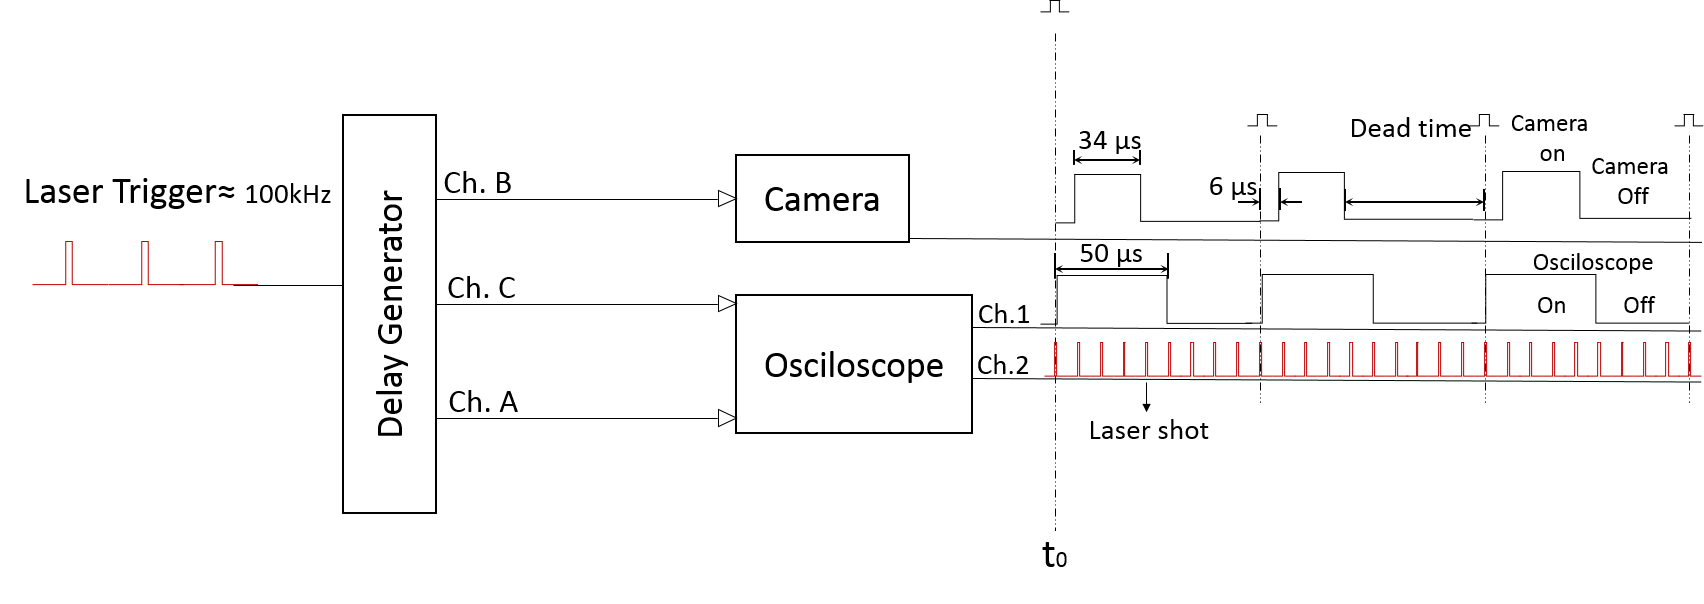
\includegraphics[width = 14 cm]{../Images/Trigger scheme.png}
\caption[Trigger Scheme]{Scheme of the trigger system used.  }
\label{fig:triggers}
\end{figure}

In Fig \ref{fig:triggers}, we show the Trigger scheme used in the experiment. The oscilloscope and camera are triggered by the delayed channel B. The oscilloscope is set to $50\mu s$ and the camera to the minimal exposure time. So the camera and oscilloscope sees the same trigger, the oscilloscope will record at least 5 laser shots, but the camera because starts later just can see three as shown. The pictures are saved in the memory RAM of the computer so the dead time after the camera is off is mandatory to give the operating system enough time to save the data on disk and don't get out of ram. A small improvement in this system can be done if we trigger the camera with B and the oscilloscope with C, so both apparatus can start almost at the same time and no corrections need to be done. Each of the data set is save with a unique label to correlate the signals after. Once an explosion is found in the VMI pictures, we check in its corresponding TOF that to proof there exist just one explosion in all five laser shots, so we can be sure that picture correspond to a single coulomb explosion, in case more than one signal is found, this picture is discarded. Fig \ref{fig:correlatesimg} shows an example of some electron-VMI pictures to its corresponding TOF. Fig A shows a typical VMI-TOf relation with one peak in the time of flight for $^{+}$He. Fig b. presents a brighter electron VMI picture meaning a bigger explosion as seen in the TOF. Fig c. show an example of a Coulomb explosion where dimmers where formed as show in the TOF with two peaks that correspond to $^{+}$He and He$^{2}$.

\begin{figure}[h!]
 \centering
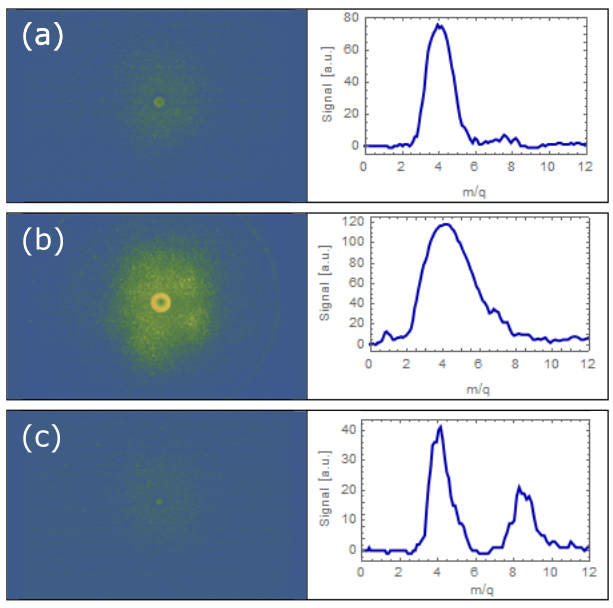
\includegraphics[width=0.6\textwidth]{../Images/results/mir_correlated/mir_correlated.png} 
  \caption[Correlation signals example]{Example of VMI-TOF correlation signals for He droplets, in the left some Electronic VMI pictures and on the right their correspondent TOF spectra On the Y-axis the Ion yield and on the x-axes the mass/charge }
  \label{fig:correlatesimg}
 \end{figure}
  

\section{Calibration Methods}

\subsection{VMI calibration}

To calibrate the VMI spectrometer, two different methods were used. A quadratic calibration function $E=\alpha\cdot r^2$ is used, where $E$ is the kinetic energy of the particles and $r$ is the measured radius. This function is chosen because $E_{kin}=1/2 \cdot m v^2$. In order to keep the simplicity, stray fields, third order or linear terms are not included, as long as the calibration curves fit well with the measured.

On one hand, the most independent method is the trajectory simulation, because it does not rely on any laser system or physical process. These simulations were done by Dominik Schomas with SIMION 8.1. For the starting conditions for the electrons we chose a small interaction volume comparable to the estimated experimental parameters and the emission direction perpendicular to the spectrometer axis. For those electrons the projected energy on the detector screen is equivalent to the real kinetic energy, with this the inverse Abel transformation can be avoided. It is necessary to simulate different kinetic energies for the electrons, at different velocity vectors. After extracting the radii, where the electrons hit the detector plane, a calibration from pixels to mm for the camera is needed, because SIMION gives the radii of the electrons in mm. To do so, known distance in the camera image is needed, for example the inner diameter of the phosphor screen, making possible to generate the fit curve. The disadvantage of this method is, that it is very difficult to include any magnetic or electric stray fields into the simulations or other external parameter that can be in reality.

\begin{figure}[h!]
\centering
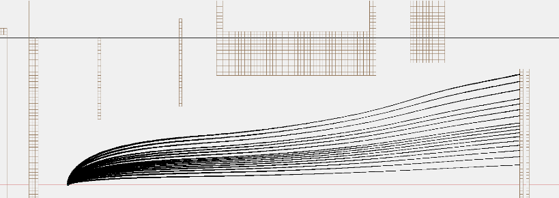
\includegraphics[scale=1]{../images/simion_calib.png}
\caption{energy calibration of the VMI spectrometer with SIMION. Electrons with discrete kinetic energy are emitted perpendicular to the spectrometer axis.}
\end{figure}


On the other hand, in order to contrast the simulation, a physical process is used, creating electrons with a well-known energy, then above threshold ionization (ATI) of rare gas atoms is a suitable method to calibrate the spectrometer. The result of the ATI mechanism are several rings in the VMI along the laser polarization axis that are energetically spaced by the energy of one photon. With at least 2 rings visible it is possible to do the calibration with the following formula

\begin{align*}
\Delta E = \alpha (r_2^2-r_1^2)
\end{align*}
where $\Delta E$ is the photon energy, $r_i$ are the peak positions of the Abel inverted rings and $\alpha$ the calibration factor. Best results are achieved by using as low peak intensities as possible, so tunnel ionization is suppressed.


Another method to calibrate a VMI spectrometer is the use of a narrowband laser in combination with resonant processes. A very useful scheme is published by \textit{Wituschek et al.} \cite{wituschek_simple_2016}. The scheme uses continuous 404 nm laser light to excite either the 5p${}_{3/2}$ or the 5p${}_{1/2}$ state in potassium. From this state, relaxation in four other states and the ground state is possible. The 404 nm light can also ionize electrons from the resonant 5p state, the 5s, the 3d and the 4p states. The resulting electrons carry a very well defined kinetic energy $E_{kin}=E_{Photon}+E_{state}-E_{ionization}$. Since all energies on the right side of the equation are well known, the kinetic energy is also well known. This allows the calibration of the spectrometer with three points (the cross section of the 5s state is too small to see it) in the low energy range.

\begin{figure}
\centering
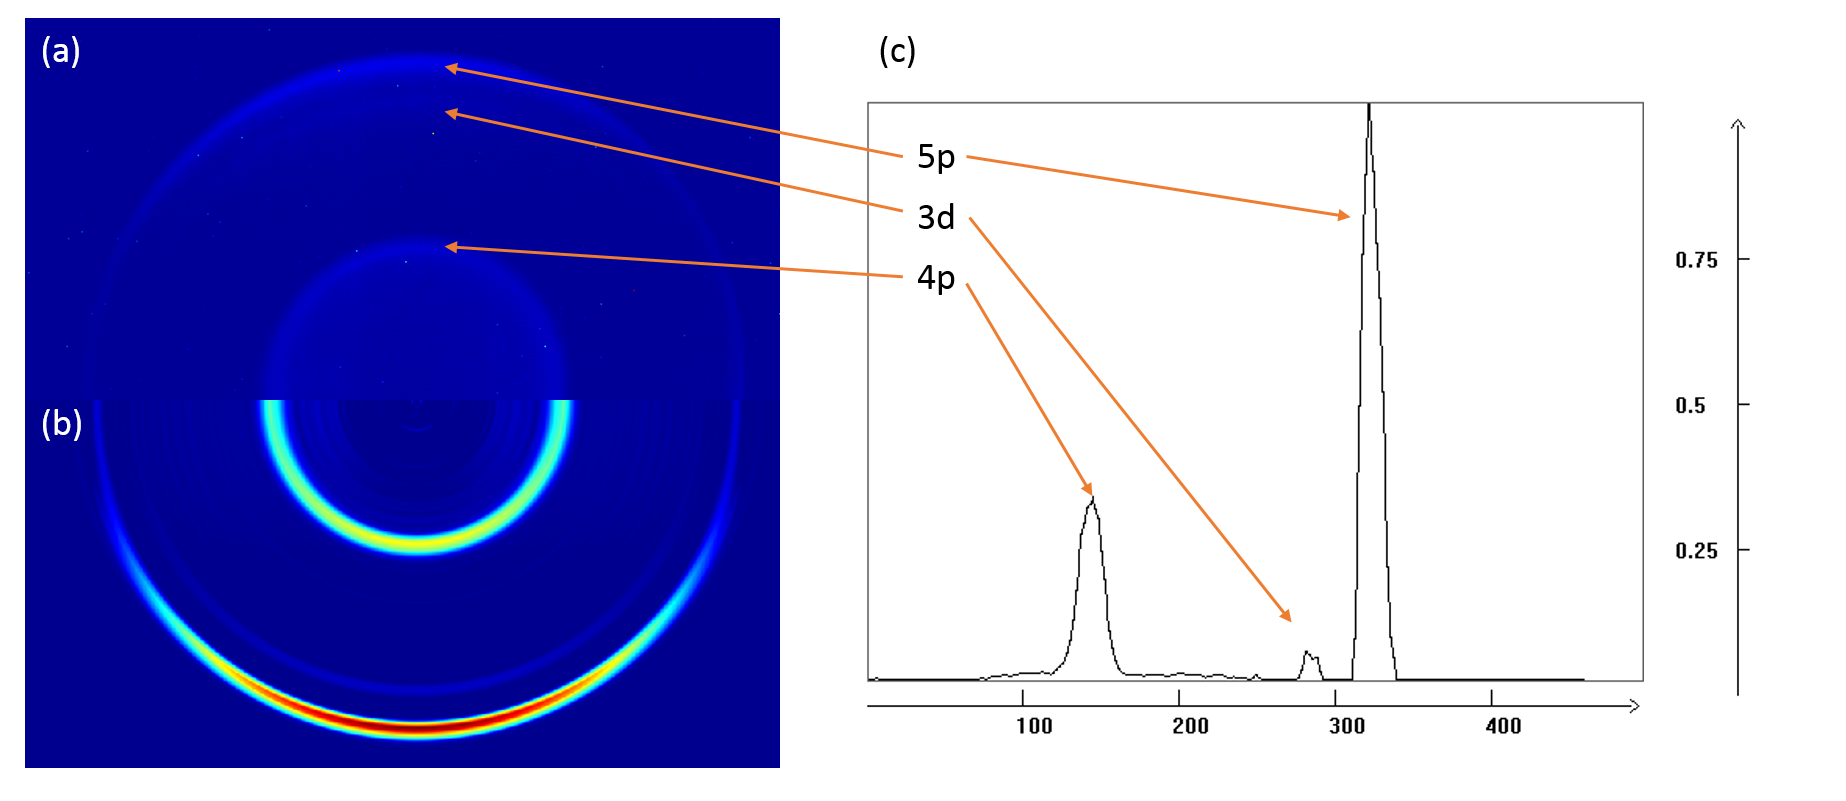
\includegraphics[scale=0.5]{../images/potassium_calib.png}
\caption{(a) Photoelectron image of potassium excited and ionized by linear polarized 404nm light, (b) Abel inverted image and (c) corresponding photoelectron spectrum, not yet calibrated on the energy}
\end{figure}


\subsection{Laser Intensity Calibration}
When using a focused MIR and NIR laser, it is essential to know the peak intensity in the focus of the laser field. Most of the time calculations give wrong results, because they assume a perfectly Gaussian shape and do not account losses in optics after the power measurement or an imperfect focus. So it would be desirable to avoid calculations and measure the peak intensity directly. In this thesis two different schemes are used, the 2U$_P$ cutoff energy of electrons in a laser field \cite{Becker_2018}, \cite{becker_vuv_1996} and the ratios of charge states of ions produced in the laser field \cite{augst_laser_1991}.

Assuming that the laser is a perfect Gaussian beams we can calculate with linear optics the Focused intensity. In cylindrical coordinates with the origin in the focus of the beam where z is the direction of propagation and $r$ the distance from the z-axis one can use following equations to describe the intensity distribution of the beam:

\begin{equation}
w_{0}=\dfrac{f\lambda}{\pi \omega}
\end{equation}
 where $w_{0}$ is the calculated focus depending on the focal length of the focsused mirror $f$, the wavelength of the laser $\lambda$ and the radius of the collimated beam before it is focused.
the intensity will red as

\begin{equation}
I_{0}=\dfrac{2P}{\pi \omega_{o}^{2}R \tau}
\end{equation} 
 where $P$
is the power of the laser, $R$ is the repetition rate and $\tau$ is the laser pulse duration.




\section{Data Analysis}

Due the complexity of the coulomb explosion, few analytical models exist in literature. the variables and parameter in which the nanoplasma depends are several and its analysis can be quite complicated. As shown above, the individual signal tends to have a well defined circular shape that can be advantageous to our analysis, Fig.  XXX shows a picture of the normalized sum several signals for helium at 10.6 K and have a similar behaiviur for the other experiments. On the left, the corresponding kinetic energy  distribution after doing the inverse Abel transform in Pbasex software. As see, there  exist a large combination of energy available along the plasma production and  can be comparable to the most recent work of \textit{Kelbr et al} \cite{kelbg_auger_2019}, where the electron spectra show  similar values.

This large range of spectra for the averaged data and the defined circularity of the individual signal make us suspect that exist a energy dependence. Fig. \ref{fig:abeltransf} show a raw picture of single event and its  Abel transform. The sharp peak in the electron spectra show a strong electron energy preference that change in each explosion. The peak in the energy distribution define the radius of the signal. To avoid doing the Inverse Abel transform for each individual picture, we create a event finder algorithm to  identify and analyse each signal in the data sets. In this way we will detect and analyse the max energy distribution in the nanoplasma for the single explosion, and correlated to the electron yield given by the intensity of the signal.
 
\begin{figure}[h!]
 \centering
 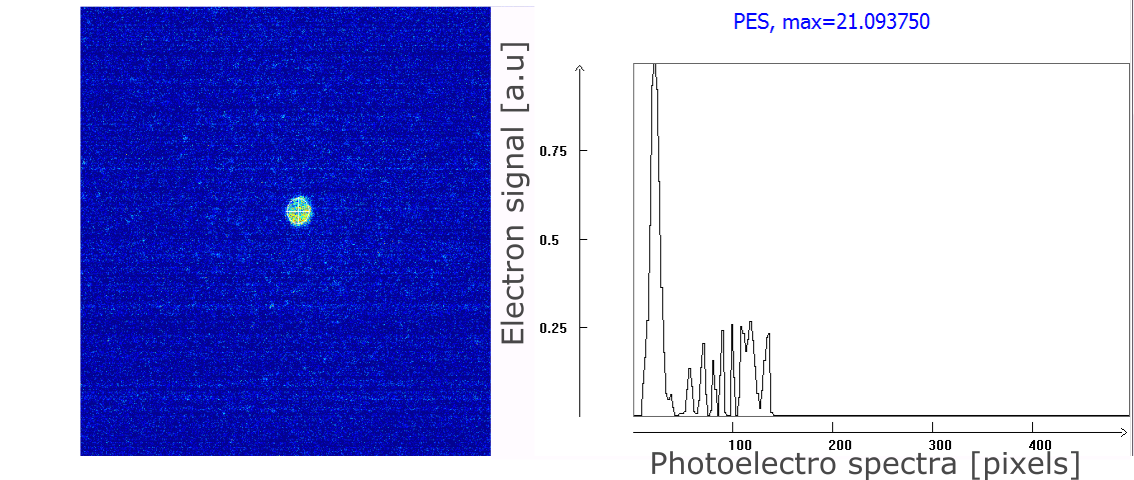
\includegraphics[width=12 cm]{../Images/abel inverse transform.png}
 \caption[Abel inverse transform example]{Example of the Inverse Abel transform for a single shot image. The photo electron spectra show the energy distribution of the signal with a peak in 21 pixels}
 \label{fig:abeltransf}
 \end{figure}
   
In other words, Our result will be based in the finding and analysis of the Max radius and brightness of each individual bloop signal. The next section shows the event recognition scheme and the radius finder  algorithm.

\subsection{Event Recognition}

The low event rate of  the nanoplasma explosion results in a lot of empty VMI images. On average 10000 pictures were taken for each set of data where less than $10\%$ of them contain signal. To separate empty images from signals, the central bright bloop is used. A center is selected manually and all pixels within a region around the center are summed up. If the sum is above a certain threshold value the image contains a signal. To analyse the central feature in more detail the size and the brightness of this feature is of importance. To determine the radius and the brightness, two methods were compared, one using the Mathematica 10.1 (wolfram inc.) algorithms and the other using a binning processing.

First, the ImageMeasurements and Componentmeasurements algorithms in Mathematica act, over binarized images, works with arbitrary 2D and 3D images and computes multiple properties, finding components bases on a specific matrix. For this special case, a circular matrix with the specifications of minimum radius and no share edges were given as parameters. The efficient of this process was demonstrated to depend strongly on the initial image and the signal-noise rate, hence, a recursive function were develop to change the binarized threshold recursively until the algorithm find just one object that matches the signal. The threshold was changed progressively and modifiable steps in order to get the most precise fit. Once the object is found, the radius and center are saved, and sum the total intensity inside the radius, so a Radius-Brightness measurement is complete for each individual image.

The second method was based on a circular binning of the signal. A center for each data set is manually place after summed all signal pictures and find the center of the signal bloop, set to be in the same position within one measurement. Three circles are defined around this center, the first one with radius $r$ (in pixels), which is variable, the second one with $r_{in} = r-\Delta r$ and the last one with $r_{out} = r + \Delta r$, where $\Delta r$ has to be picked out from the dataset. The three circles define two areas $A_{in}$ and $A_{out}$, see Fig  \ref{fig:density_plot}. An average pixel value $\rho$ for both areas is defined via

\begin{align}
\rho_{in} & = \frac{1}{N_{in}} \sum_{px \in A_{in}} \text{value}(px) - bg \\
\rho_{out} & = \frac{1}{N_{out}} \sum_{px \in A_{out}} \text{value} (px) -bg \\
\end{align}

Where $N$ is the number of pixels in the respective area and $bg$ is a background taken far from the central features. The normalization on the area is important, because the areas are of different size. To finally find out the radius of the central circle, the difference $\rho_{in}-\rho_{in}$ is maximized, this is the case for the orange box in figure \ref{fig:density_plot}. For the green and the purple boxes $\rho_{in} = \rho_{in}$, which gives zero for the difference.
Real signals do not have a perfect cut-off or a constant radial profile, which leads to noisy curves, when $\Delta r$ is chosen too small, which makes the determination of $r$ difficult. An example of a single shot image, where the radius is determined for $\Delta r = 3,4,5$ in pixels, is shown in figure \ref{fig:density_plot}. The VMI image in this figure has a donut shape, if the inner radius is of interest the same curve can be used to determine the inner radius as well if the minimum of the function is taken.
\begin{figure}

\centering
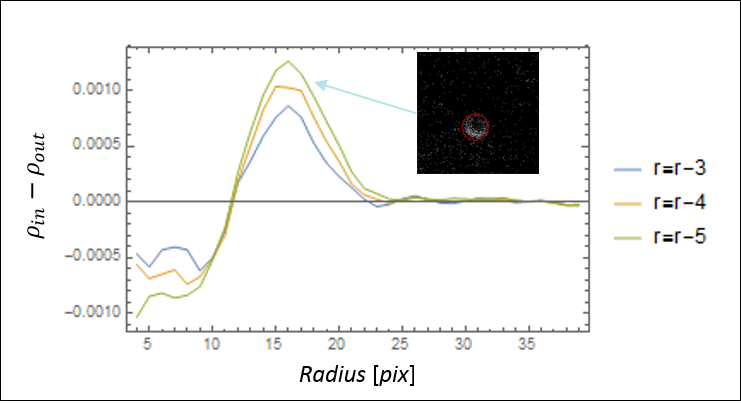
\includegraphics[width=10 cm]{../images/density_plot.png}
\caption{Difference of mean pixel values to determine the radius of the central feature in the VMI images}
\label{fig:density_plot}
\end{figure}

As shown in \ref{fig:density_plot}, the density difference have a summit in two cases, one when the inner our outer density changes signs. The lower peak, when exists, refers to the change from a low density change to a high one, besides the higher peak, describe the change from a high density to a lower, setting the radius where the edge of the bloop is pointing out that not all signals have the donut shape so this case was just added when needed. Finally, as in the last procedure, the inner pixels in the circle with radius $r$ are summed and the radius-Brightness is save for all signal. In the case, as the example, where the second inner circle is clearly identified, the sum of all the pixel discard the inner are, and at the same time, adds the inner radius-brightness measurements to it. 
Fig \ref{fig:abelfinder} shows a raw image where the inverse Abel transform and the Binned Finder algorithms where compare. The signal shows a clear edge where the peak electron signal (PES) of the Abel transform is at 58.6 pixels, while a similar curve is described by the density binned plot of the Finder algorithm at 60 pix, given a good agreement between the two techniques.
Figure \ref{fig:checkradius} shows a set of well fitted radius for each signal, proving the good efficiency of the algorithms. 

\begin{figure}[hbtp!]
\centering
\begin{subfigure}[l]{1\textwidth}
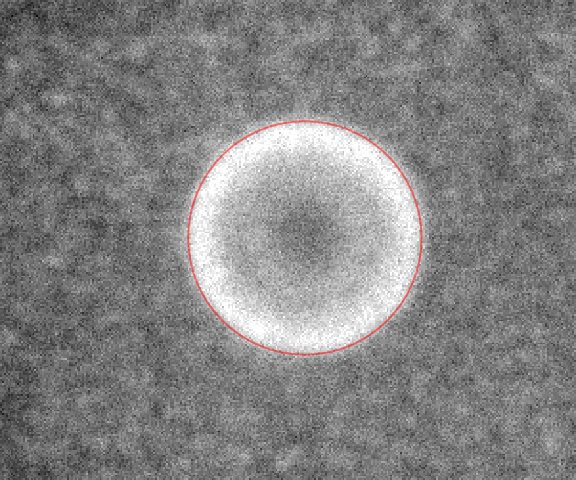
\includegraphics[width=0.4\textwidth]{../Images/rawVMIfit.PNG} 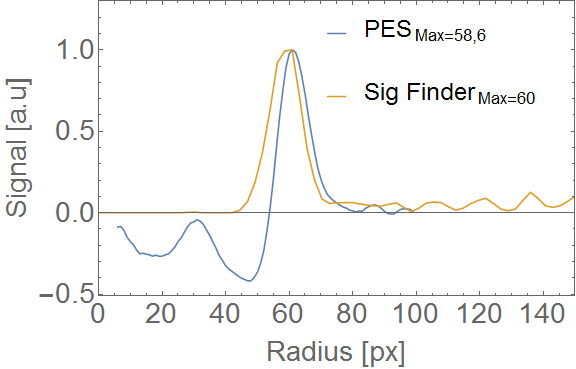
\includegraphics[width=0.5\textwidth]{../Images/pesandFinder.PNG} \end{subfigure} 
\caption[Fit-Abel transform agreement]{On the Left, example images of MIR VMI signal. On the right, the correspond Inverse Abel transform PES (orange) and the Bloop finder density plot (blue). Both algorithms show a peak at radius of the circular signal, highlighted in red. The density plot also shows a second depletion close to 45 pixel that give extra information as the radius of the inner less brighter ring. }
\label{fig:abelfinder}
\end{figure}


\begin{figure}[hbtp]
\caption[Example signal finder]{Example of random signal images fitted to its corresponding radius.}
\centering
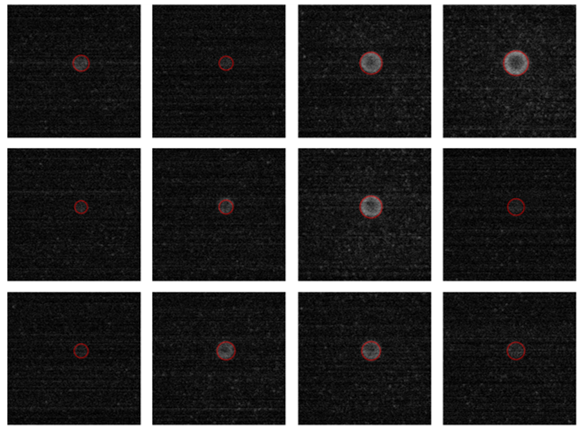
\includegraphics[width=10cm]{../Images/density_plot_chekc.png}
\label{fig:checkradius}
\end{figure}
Last, once the radius-brightness data is recorded, and the calibrations are set, the system can be compare to the model explained above, where radius can be converted into maximal kinetic energy, $r\rightarrow k_{energy}$, and brightness to number of electrons, $b\rightarrow N_{e-}$. 


